\chapter[Capire il Problema: Leggere da Programmatore]{Capire il Problema:\\ Leggere da Programmatore}
\label{chap:comprensione}

\begin{quote}
\itshape
\small
``Il computer fa esattamente quello che gli diciamo. Se leggiamo male il testo, il bug nasce prima ancora di disegnare il primo blocco.''
\end{quote}
\vspace{1em}

\noindent\textbf{Riferimento Lezione:} 12 Ottobre 2026 -- Quarta Lezione di Laboratorio\\
\textbf{Progetto Guida Annuale:} \textbf{\color{PiazzaPrimary}Mars City Builder (Lite)}\\
\textbf{Competenze chiave:} Lettura attiva del testo di un problema, separazione tra dati, richiesta, regole e rumore, traduzione delle parole in confronti, compilazione della scheda I-P-O e verifica del caso limite.

\vspace{1.5em}

\noindent In questo capitolo non scriviamo né codice né pseudocodice: impariamo a \textbf{capire} il problema, che è il passo che viene prima di tutti gli altri.

% ------------------------------------------------------------------------------
\section{Perché Leggere Prima di Risolvere?}
% ------------------------------------------------------------------------------

\begin{attenzione}[Il Bug Nato da Due Parole]
Il testo dice: \emph{``L'allarme deve suonare quando restano \textbf{al massimo 10} unità di ossigeno.''}\\
Il programmatore frettoloso capisce: \emph{``L'allarme suona quando restano \textbf{meno di 10} unità.''}

\smallskip
Con esattamente 10 unità il testo vuole l'allarme ($10 \leq 10$ è VERO), il programma invece tace ($10 < 10$ è FALSO). Nessun errore di calcolo: solo una lettura sbagliata.
\end{attenzione}

% ------------------------------------------------------------------------------
\section{Lo Schema I-P-O come Filtro di Lettura}
% ------------------------------------------------------------------------------

Lo schema I-P-O (Capitolo~\ref{chap:sequenza}) non serve solo a progettare: è anche un \textbf{filtro} per leggere. A ogni frase del testo chiediamo in quale casella va.

\begin{center}
\renewcommand{\arraystretch}{1.45}
\begin{tabular}{|l|l|p{6.6cm}|}
\hline
\rowcolor{PiazzaPrimary!15}
 & \textbf{Domanda da farsi} & \textbf{Cosa cercare nel testo} \\
\hline
\textbf{\color{BoxBlue}INPUT} & Cosa mi \textbf{dai}? & I dati noti: numeri, quantità, misure. \\
\hline
\textbf{\color{BoxAmber}ELABORAZIONE} & Quali \textbf{regole}? & Calcoli e condizioni che collegano dati e risultato. \\
\hline
\textbf{\color{PiazzaPrimary}OUTPUT} & Cosa mi \textbf{chiedi}? & Il risultato da trovare o il messaggio da mostrare. \\
\hline
\end{tabular}
\end{center}

\begin{concetto}[Il Rumore]
Tutto quello che non entra in nessuna casella è \textbf{rumore}: nomi, orari, colori, emozioni. Rende bella la storia, ma il computer non lo usa. A volte il rumore è perfino un \textbf{numero}.
\end{concetto}

% ------------------------------------------------------------------------------
\section{Il Metodo del Programmatore in 5 Passi}
% ------------------------------------------------------------------------------

\begin{enumerate}
  \item \textbf{Leggi due volte.} La prima volta per capire la storia, la seconda per cercare i dati.
  \item \textbf{Evidenzia} con i colori o con i simboli del kit (Sezione~\ref{sec:kit-prima}).
  \item \textbf{Riformula} con una sola frase: \emph{``Devo capire se\dots''}.
  \item \textbf{Compila la scheda I-P-O} sul quaderno: riformulazione, input, elaborazione, output.
  \item \textbf{Prova a mano} con i numeri del testo e poi con il \textbf{caso limite}.
\end{enumerate}

\begin{concetto}[Regola d'Oro]
Nessuna soluzione finché non hai completato i 5 passi.
\end{concetto}

% ------------------------------------------------------------------------------
\section{Il Kit dell'Evidenziatore: Colori e Simboli}
\label{sec:kit-prima}
% ------------------------------------------------------------------------------

Chi ha gli evidenziatori usa \textbf{colore e simbolo insieme}. Chi non li ha usa \textbf{solo il simbolo}, con una penna qualsiasi: ogni simbolo si disegna a mano in un secondo.

\begin{center}
\renewcommand{\arraystretch}{1.6}
\begin{tabular}{|l|l|l|p{4.2cm}|}
\hline
\rowcolor{PiazzaPrimary!15}
\textbf{Cosa cerco} & \textbf{Colore} & \textbf{Come appare} & \textbf{Simbolo a mano} \\
\hline
Dato (Input)       & blu    & \dato{40 unità}            & \textbf{cerchio}: cattura il dato \\
\hline
Richiesta (Output) & rosso  & \richiesta{serra riparata?} & \textbf{doppia sottolineatura}: il risultato \\
\hline
Regola             & giallo & \regola{se basta}           & \textbf{onda}: il bivio, la strada cambia \\
\hline
Rumore             & ---    & \rumore{il tecnico Rossi}   & \textbf{barrato}: lo butto via \\
\hline
Dato nascosto      & blu    & \nascosto{7 giorni}         & \textbf{$\bigstar$ a margine} + il dato \\
\hline
Dato mancante      & ---    & \mancante{metallo}          & \textbf{? a margine} + la domanda \\
\hline
\end{tabular}
\end{center}

Quando una regola contiene un confronto, lo scriviamo accanto: \regola{se il cibo basta}\confronto{$\geq$}.

% ------------------------------------------------------------------------------
\section{Il Dizionario: Parole che Diventano Confronti}
% ------------------------------------------------------------------------------

\begin{center}
\renewcommand{\arraystretch}{1.4}
\begin{tabular}{|l|c|l|l|}
\hline
\rowcolor{PiazzaPrimary!15}
\textbf{Parola nel testo} & \textbf{Confronto} & \textbf{Esempio} & \textbf{La soglia è\dots} \\
\hline
almeno                & $\geq$ & ``almeno 50 di metallo''              & compresa \\
al massimo            & $\leq$ & ``al massimo 6 coloni''               & compresa \\
più di / supera       & $>$    & ``supera 120 km/h''                   & esclusa \\
meno di / sotto       & $<$    & ``meno di 40 punti''                  & esclusa \\
fino a                & $\leq$ & ``resiste fino a 120 km/h''           & compresa \\
basta / è sufficiente & $\geq$ & ``il cibo basta''                     & compresa \\
esattamente / pari a  & $=$    & ``esattamente 10 coloni''             & solo quella \\
diverso da / tranne   & $\neq$ & ``tutti tranne il rover 2''           & esclusa \\
\hline
\end{tabular}
\end{center}

\begin{attenzione}[Il Caso Limite]
Prova sempre con il numero \textbf{esatto} della soglia (50, 120, 10\dots). È lì che ``almeno'' e ``più di'' danno risultati opposti, ed è lì che si nasconde il bug.
\end{attenzione}

% ------------------------------------------------------------------------------
\section{Le 4 Trappole del Testo}
% ------------------------------------------------------------------------------

\begin{enumerate}
  \item \textbf{Il rumore:} nomi, orari e perfino numeri che non servono (\emph{``la serra ha perso il 40\% delle piante''}).
  \item \textbf{Il dato nascosto:} il testo non lo scrive, ma serve (\emph{``per una settimana''} $\to$ $\bigstar$ 7 giorni).
  \item \textbf{Le parole-trappola:} ``almeno'' e ``più di'' sembrano uguali, ma sul caso limite danno risultati opposti.
  \item \textbf{Il dato mancante:} un'informazione indispensabile non c'è. Non si inventa: si scrive \textbf{?} e la domanda da fare.
\end{enumerate}

% ------------------------------------------------------------------------------
\newpage
\section{Esempio Svolto: Il Turno dell'Ossigeno}
% ------------------------------------------------------------------------------

\begin{center}
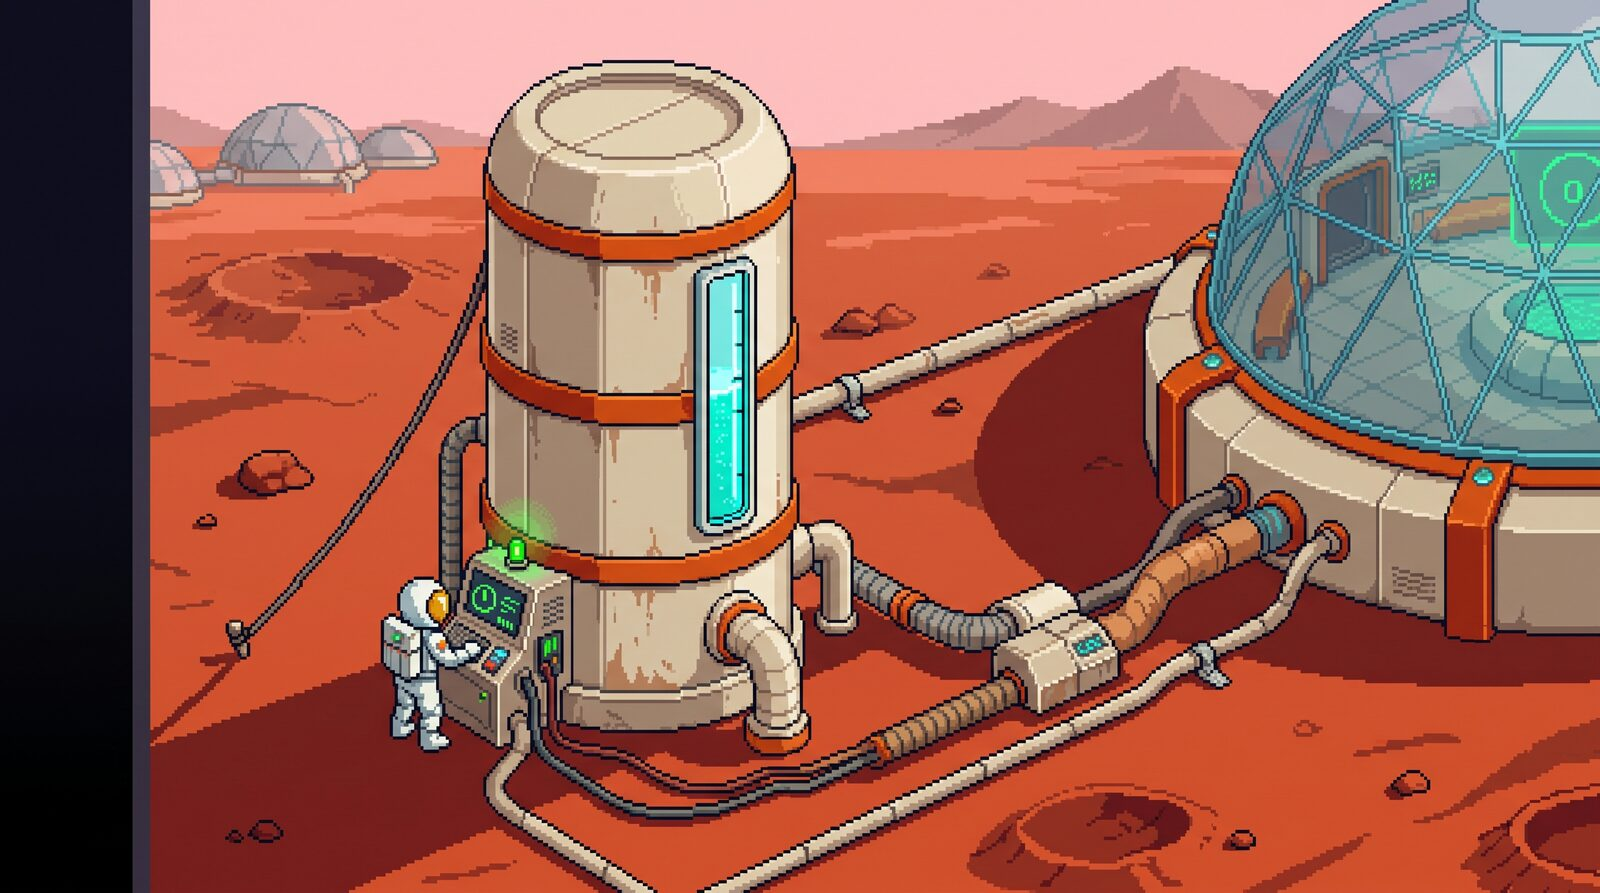
\includegraphics[width=0.8\textwidth]{../2026-10-12/presentazione/immagini/ossigeno.jpeg}
\end{center}

\begin{esempio}[Il Testo]
\emph{Sono le 6:40 del mattino nella Colonia Alpha-1 e la sirena del cambio turno ha appena suonato. Il tecnico Rossi, arrivato su Marte da appena tre settimane, controlla il pannello del generatore. Ogni colono consuma 3 unità di ossigeno al giorno. Il serbatoio contiene 40 unità e nella colonia vivono 12 coloni. Se l'ossigeno del serbatoio basta per tutta la giornata, il pannello deve mostrare ``Respirate tranquilli''; altrimenti deve far scattare l'allarme rosso. Cosa deve mostrare il pannello oggi?}
\end{esempio}

\begin{soluzione}[Il Testo Annotato e la Scheda I-P-O]
\rumore{Sono le 6:40 del mattino nella Colonia Alpha-1 e la sirena del cambio turno ha appena suonato.} \rumore{Il tecnico Rossi, arrivato su Marte da appena tre settimane,} controlla il pannello del generatore. Ogni colono consuma \dato{3 unità} di ossigeno al giorno. Il serbatoio contiene \dato{40 unità} e nella colonia vivono \dato{12 coloni}. \regola{Se l'ossigeno del serbatoio basta}\confronto{$\geq$} per tutta la giornata, il pannello deve mostrare \richiesta{``Respirate tranquilli''}; \regola{altrimenti} deve far scattare \richiesta{l'allarme rosso}. \richiesta{Cosa deve mostrare il pannello oggi?}

\begin{scheda}
Riformulo & \emph{``Devo capire se l'ossigeno basta per tutti i coloni di oggi.''} \\ \hline
Input & ossigeno nel serbatoio = \textbf{40} \textbullet{} coloni = \textbf{12} \textbullet{} consumo a testa = \textbf{3} \\ \hline
Elaborazione & fabbisogno = coloni $\times$ 3 \newline basta? $\to$ serbatoio $\geq$ fabbisogno \\ \hline
Output & ``Respirate tranquilli'' \textbf{oppure} allarme rosso \\ \hline
Prova a mano & $12 \times 3 = 36$ $\to$ $40 \geq 36$ \textbf{VERO} $\to$ ``Respirate tranquilli'' \newline Caso limite: serbatoio = 36 $\to$ $36 \geq 36$ $\to$ basta ancora! \\ \hline
\end{scheda}
\end{soluzione}

% ------------------------------------------------------------------------------
\newpage
\section{Le 5 Sfide del Programmatore}
% ------------------------------------------------------------------------------

Modalità: \textbf{a coppie}. Su ogni testo evidenzia con colori o simboli. Sul quaderno scrivi la frase \emph{``Devo capire se\dots''}, la scheda I-P-O e la prova a mano con il caso limite.

\begin{esercizio}[Sfida 1: La Tempesta di Sabbia]
Il radar meteo della base Tharsis segnala una tempesta di sabbia in arrivo da nord-ovest, a 380 chilometri di distanza. Le raffiche sollevano la polvere rossa fino a 2 chilometri di altezza. La comandante Okafor, al suo secondo anno di missione, posa il caffè liofilizzato e ordina di controllare gli scudi. Gli scudi della cupola resistono a venti fino a 120 km/h; il radar stima che la tempesta soffierà a 135 km/h. Se il vento supera la resistenza degli scudi, i coloni devono rifugiarsi nel bunker; altrimenti possono restare nelle cupole. Dove devono andare i coloni?
\end{esercizio}

\begin{esercizio}[Sfida 2: Razioni per la Settimana]
La navetta cargo Ares-3 è atterrata ieri sera sulla pista n.~2, ma il comandante vuole sapere se il cibo in magazzino basta per una settimana intera, senza aspettare il prossimo rifornimento. Nella colonia vivono 10 coloni e ognuno mangia 2 razioni al giorno. Nel magazzino ci sono 150 razioni. Le razioni preferite dai coloni sono quelle alla soia affumicata. Se il cibo non basta, bisogna ordinare un rifornimento urgente dalla Terra. Serve il rifornimento?
\end{esercizio}

\begin{esercizio}[Sfida 3: La Fabbrica di Mattoni]
Il consiglio della colonia ha votato all'unanimità: è arrivato il momento di accendere la nuova fabbrica di mattoni. Per partire, la fabbrica ha bisogno di almeno 50 unità di energia libera. La centrale solare produce 200 unità, mentre gli edifici già accesi ne consumano 150. Se l'energia libera è meno di 50, la fabbrica resta spenta e i muratori tornano a giocare a carte nella mensa; altrimenti la fabbrica si accende. La fabbrica si accende?
\end{esercizio}

\begin{esercizio}[Sfida 4: Il Nuovo Quartiere]
Con l'ultima navetta sono arrivati 9 nuovi coloni che non hanno ancora un letto. Il sindaco Hernández, che ama i nomi poetici, ha già deciso di chiamare il nuovo quartiere ``Valle dell'Alba''. Ogni modulo abitativo ospita al massimo 6 coloni e costa 80 unità di metallo. Se il metallo in magazzino basta, si costruiscono tutti i moduli necessari; altrimenti i nuovi coloni dormono nella palestra della base. Quanti moduli servono? Si possono costruire?
\end{esercizio}

\begin{esercizio}[Sfida 5: Il Meteorite sulla Serra]
Durante la lunga notte marziana, mentre la colonia dorme, un piccolo meteorite colpisce la serra idroponica. L'ingegnera capo Lindqvist, svegliata dall'allarme, corre a controllare in tuta pressurizzata: la serra ha perso il 40\% delle piante e 4 pannelli di vetro sono in frantumi. Riparare un pannello costa 30 unità di metallo. Se il metallo in magazzino è almeno pari al costo della riparazione, la serra viene riparata subito; se invece non basta, la serra resta chiusa fino al prossimo rifornimento. In magazzino ci sono 100 unità di metallo. La serra verrà riparata?
\end{esercizio}

\begin{consiglio}[La Scheda I-P-O da Copiare sul Quaderno]
\begin{scheda}
Riformulo & Devo capire se \dotfill \\ \hline
Input & (nome = valore) \\ \hline
Elaborazione & (calcoli e confronti) \\ \hline
Output & \\ \hline
Prova a mano & (+ caso limite) \\ \hline
\end{scheda}
\end{consiglio}

% ------------------------------------------------------------------------------
\newpage
\section{Soluzioni Commentate}
% ------------------------------------------------------------------------------

\begin{soluzione}[Sfida 1: La Tempesta di Sabbia --- trappola: il rumore]
\rumore{Il radar meteo della base Tharsis segnala una tempesta di sabbia in arrivo da nord-ovest, a 380 chilometri di distanza. Le raffiche sollevano la polvere rossa fino a 2 chilometri di altezza. La comandante Okafor, al suo secondo anno di missione, posa il caffè liofilizzato e} ordina di controllare gli scudi. Gli scudi della cupola resistono a venti \regola{fino a}\confronto{$\leq$} \dato{120 km/h}; il radar stima che la tempesta soffierà a \dato{135 km/h}. \regola{Se il vento supera la resistenza degli scudi}\confronto{$>$}, i coloni devono rifugiarsi \richiesta{nel bunker}; \regola{altrimenti} possono restare \richiesta{nelle cupole}. \richiesta{Dove devono andare i coloni?}

\begin{scheda}
Riformulo & \emph{``Devo capire se il vento è più forte di quanto reggono gli scudi.''} \\ \hline
Input & resistenza scudi = \textbf{120 km/h} \textbullet{} velocità del vento = \textbf{135 km/h} \\ \hline
Elaborazione & ``supera'' $\to$ vento $>$ resistenza \\ \hline
Output & ``Tutti nel bunker'' \textbf{oppure} ``Restate nelle cupole'' \\ \hline
Prova a mano & $135 > 120$ \textbf{VERO} $\to$ tutti nel bunker! \newline Caso limite: vento = 120 $\to$ $120 > 120$ FALSO $\to$ gli scudi reggono (``fino a''). \\ \hline
\end{scheda}
Anche i 380 km e i 2 km sono rumore: sono numeri, ma non entrano in nessuna casella.
\end{soluzione}

\begin{soluzione}[Sfida 2: Razioni per la Settimana --- trappola: il dato nascosto]
\rumore{La navetta cargo Ares-3 è atterrata ieri sera sulla pista n.~2,} ma il comandante vuole sapere se il cibo in magazzino \regola{basta}\confronto{$\geq$} per \dato{una settimana intera}\nascosto{7 giorni}, senza aspettare il prossimo rifornimento. Nella colonia vivono \dato{10 coloni} e ognuno mangia \dato{2 razioni al giorno}. Nel magazzino ci sono \dato{150 razioni}. \rumore{Le razioni preferite dai coloni sono quelle alla soia affumicata.} \regola{Se il cibo non basta}\confronto{$<$}, bisogna \richiesta{ordinare un rifornimento urgente dalla Terra}. \richiesta{Serve il rifornimento?}

\begin{scheda}
Riformulo & \emph{``Devo capire se 150 razioni coprono 7 giorni per tutti i coloni.''} \\ \hline
Input & razioni = \textbf{150} \textbullet{} coloni = \textbf{10} \textbullet{} razioni a testa al giorno = \textbf{2} \textbullet{} $\bigstar$ giorni = \textbf{7} \\ \hline
Elaborazione & fabbisogno = coloni $\times$ 2 $\times$ 7 \newline basta? $\to$ razioni $\geq$ fabbisogno \\ \hline
Output & ``Nessun rifornimento'' \textbf{oppure} ``Rifornimento urgente!'' \\ \hline
Prova a mano & $10 \times 2 \times 7 = 140$ $\to$ $150 \geq 140$ \textbf{VERO} $\to$ nessun rifornimento. \\ \hline
\end{scheda}
Senza il $\bigstar$ si calcola $10 \times 2 = 20$ e si arriva alla stessa risposta per il motivo sbagliato: con 130 razioni il calcolo corretto fa scattare il rifornimento, quello sbagliato no.
\end{soluzione}

\begin{soluzione}[Sfida 3: La Fabbrica di Mattoni --- trappola: le parole-trappola]
\rumore{Il consiglio della colonia ha votato all'unanimità: è arrivato il momento di} accendere la nuova fabbrica di mattoni. Per partire, la fabbrica ha bisogno di \regola{almeno}\confronto{$\geq$} \dato{50 unità} di energia libera. La centrale solare produce \dato{200 unità}, mentre gli edifici già accesi ne consumano \dato{150}\calcolo{libera = 200 $-$ 150}. \regola{Se l'energia libera è meno di}\confronto{$<$} 50, la fabbrica \richiesta{resta spenta} \rumore{e i muratori tornano a giocare a carte nella mensa}; \regola{altrimenti} la fabbrica \richiesta{si accende}. \richiesta{La fabbrica si accende?}

\begin{scheda}
Riformulo & \emph{``Devo capire se l'energia che avanza arriva ad almeno 50.''} \\ \hline
Input & produzione = \textbf{200} \textbullet{} consumo = \textbf{150} \textbullet{} soglia = \textbf{50} \\ \hline
Elaborazione & energia libera = produzione $-$ consumo \newline ``almeno'' $\to$ libera $\geq$ 50 (il contrario: libera $<$ 50) \\ \hline
Output & ``Fabbrica accesa'' \textbf{oppure} ``Fabbrica spenta'' \\ \hline
Prova a mano & $200 - 150 = 50$ $\to$ $50 \geq 50$ \textbf{VERO} $\to$ si accende! \newline Chi ha letto ``più di 50'': $50 > 50$ FALSO $\to$ fabbrica spenta. Bug! \\ \hline
\end{scheda}
\end{soluzione}

\begin{soluzione}[Sfida 4: Il Nuovo Quartiere --- trappola: il dato mancante]
Con l'ultima navetta sono arrivati \dato{9 nuovi coloni} che non hanno ancora un letto. \rumore{Il sindaco Hernández, che ama i nomi poetici, ha già deciso di chiamare il nuovo quartiere ``Valle dell'Alba''.} Ogni modulo abitativo \regola{ospita al massimo}\confronto{$\leq$} \dato{6 coloni} e costa \dato{80 unità} di metallo. \regola{Se il metallo in magazzino basta}\confronto{$\geq$}\mancante{quanto metallo c'è?}, si costruiscono \richiesta{tutti i moduli necessari}; \regola{altrimenti} i nuovi coloni \richiesta{dormono nella palestra della base}. \richiesta{Quanti moduli servono? Si possono costruire?}

\begin{scheda}
Riformulo & \emph{``Devo capire quanti moduli servono per 9 coloni e se ho il metallo per costruirli.''} \\ \hline
Input & coloni = \textbf{9} \textbullet{} posti a modulo = \textbf{6} \textbullet{} costo = \textbf{80} \newline metallo in magazzino = \textbf{? MANCA} \\ \hline
Elaborazione & 1 modulo = 6 posti (non basta) $\to$ servono \textbf{2 moduli} \newline costo = $2 \times 80 = 160$ $\to$ metallo $\geq$ 160 \\ \hline
Output & numero di moduli (2) + ``Costruiti'' \textbf{oppure} ``Tutti in palestra'' \\ \hline
Domanda da fare & Non posso rispondere! Chiedo al sindaco: \textbf{quanto metallo c'è in magazzino?} \newline Se fossero 200 $\to$ $200 \geq 160$ $\to$ 2 moduli costruiti. \\ \hline
\end{scheda}
La risposta corretta è: \emph{``Servono 2 moduli, ma non posso dire se si possono costruire.''} Inventare il dato mancante è un errore, anche se il risultato sembra plausibile.
\end{soluzione}

\begin{soluzione}[Sfida 5: Il Meteorite sulla Serra --- tutte le trappole]
\rumore{Durante la lunga notte marziana, mentre la colonia dorme,} un piccolo meteorite colpisce la serra idroponica. \rumore{L'ingegnera capo Lindqvist, svegliata dall'allarme, corre a controllare in tuta pressurizzata: la serra ha perso il 40\% delle piante} e \dato{4 pannelli} di vetro sono in frantumi. Riparare un pannello costa \dato{30 unità} di metallo\calcolo{costo = 4 $\times$ 30}. \regola{Se il metallo in magazzino è almeno pari}\confronto{$\geq$} al costo della riparazione, la serra \richiesta{viene riparata subito}; \regola{se invece non basta}\confronto{$<$}, la serra \richiesta{resta chiusa} fino al prossimo rifornimento. In magazzino ci sono \dato{100 unità} di metallo. \richiesta{La serra verrà riparata?}

\begin{scheda}
Riformulo & \emph{``Devo capire se il metallo basta per riparare tutti i pannelli rotti.''} \\ \hline
Input & pannelli rotti = \textbf{4} \textbullet{} costo a pannello = \textbf{30} \textbullet{} metallo in magazzino = \textbf{100} \\ \hline
Elaborazione & costo riparazione = pannelli $\times$ 30 \newline ``almeno pari'' $\to$ metallo $\geq$ costo \\ \hline
Output & ``Serra riparata'' \textbf{oppure} ``Serra chiusa'' \\ \hline
Prova a mano & $4 \times 30 = 120$ $\to$ $100 \geq 120$ \textbf{FALSO} $\to$ serra chiusa. \newline Caso limite: metallo = 120 $\to$ $120 \geq 120$ $\to$ riparata! \\ \hline
\end{scheda}
Il 40\% è un \textbf{numero esca}: sembra importante, ma non entra in nessun calcolo. Domanda bonus: quanto metallo manca? $120 - 100 = 20$ unità.
\end{soluzione}

% ------------------------------------------------------------------------------
\section{Errori Tipici e Checklist del Programmatore}
% ------------------------------------------------------------------------------

\begin{attenzione}[Gli Errori Più Comuni]
\begin{itemize}
  \item Partire a risolvere dopo una sola lettura.
  \item Cerchiare \textbf{tutti} i numeri, anche il 40\% e i 380 km.
  \item Dimenticare il dato nascosto (i 7 giorni).
  \item Leggere ``almeno'' come ``più di''.
  \item Inventare un dato mancante invece di chiederlo.
\end{itemize}
\end{attenzione}

\begin{consiglio}[La Checklist da Usare Prima di Ogni Flow Chart]
\begin{itemize}
  \item[$\square$] Ho letto il testo \textbf{due volte}?
  \item[$\square$] Ho \textbf{barrato} il rumore, anche i numeri che non servono?
  \item[$\square$] Ogni dato ha un \textbf{nome} e un \textbf{valore}?
  \item[$\square$] Ho trovato la \textbf{richiesta} (doppia sottolineatura)?
  \item[$\square$] Ho cercato i \textbf{dati nascosti} ($\bigstar$) e quelli \textbf{mancanti} (?)?
  \item[$\square$] Ho tradotto le regole in \textbf{confronti} ($\geq$, $>$, $\leq$, $<$, $=$, $\neq$)?
  \item[$\square$] Ho provato con i numeri del testo e con il \textbf{caso limite}?
\end{itemize}
\end{consiglio}

\begin{esercizio}[Biglietto d'Uscita: Il Rover Esploratore]
Il rover Curiosity-2, verniciato di arancione, consuma 5 unità di energia per ogni uscita e ha la batteria carica a 18 unità. Il comandante vuole sapere se il rover può fare almeno 3 uscite prima di ricaricarsi.
\end{esercizio}

\begin{soluzione}[Biglietto d'Uscita: Il Rover Esploratore]
Il rover \rumore{Curiosity-2, verniciato di arancione,} consuma \dato{5 unità} di energia per ogni uscita e ha la batteria carica a \dato{18 unità}. Il comandante vuole sapere \richiesta{se il rover può fare} \regola{almeno}\confronto{$\geq$} \dato{3 uscite} \richiesta{prima di ricaricarsi}.

\begin{scheda}
Riformulo & \emph{``Devo capire se 18 unità bastano per 3 uscite.''} \\ \hline
Input & batteria = \textbf{18} \textbullet{} consumo a uscita = \textbf{5} \textbullet{} uscite = \textbf{3} \\ \hline
Elaborazione & energia necessaria = uscite $\times$ 5 $\to$ batteria $\geq$ necessaria \\ \hline
Output & ``Sì, può partire'' \textbf{oppure} ``No, prima ricarica'' \\ \hline
Prova a mano & $3 \times 5 = 15$ $\to$ $18 \geq 15$ \textbf{VERO} $\to$ sì, può fare 3 uscite. \\ \hline
\end{scheda}
\end{soluzione}
